\fancypagestyle{plain}{%
    \fancyhf{}
    \fancyhead[RO,LE]{\bfseries \thepage}
    \fancyhead[CO]{\rightmark}
    \fancyhead[CE]{\leftmark}
    \renewcommand{\headrulewidth}{0.4pt}}

\chapter{SU(N) grupe i fizika elementarnih čestica}

Svi primjeri simetrija razmatranih u prošla tri poglavlja,
bavili su se \emph{prostorno-vremenskim} transformacijama fizikalnih
sustava, poput translacija ili rotacija. U zadnjem poglavlju knjige
bavit ćemo se Lorentzovim, Poincar\'{e}ovim i konformnim
transformacijama, koje također spadaju u kategoriju prostorno-vremenskih simetrija.
Međutim u fizici, a posebice u fizici elementarnih čestica,
od velikog su značaja i tzv. \emph{interne} simetrije, koje
djeluju na značajke čestica poput njihove vrste, električnog
naboja ili nekih "kvantnih brojeva" koji opisuju
ponašanje čestica obzirom na  slabe i jake sile.
Povijesno su istraživači nailazili na mnoge teškoće u formuliranju
ispravnih teorija tih sila koje vladaju subnuklearnim svijetom,
a i dan danas npr. ne znamo riješiti jednadžbe
gibanja koje su posljedica jake sile. Tu su se svojstva simetrija
opaženih u procesima s elementarnim česticama pokazala kao izuzetno korisna.
Najveći trijumf fizike visokih energija druge polovice XX. i početka
XXI. stoljeća je finalizacija tzv. \emph{standardnog modela} fizike elementarnih
čestica čija je struktura praktički potpuno određena njegovom
tzv. baždarnom simetrijom i odgovarajućom grupom $\SU{3} \otimes \SU{2} \otimes \U{1}$. 
Baždarne simetrije u fizici nisu tema ove knjige, ali u ovom ćemo poglavlju
objasniti neke ideje i upotrebu općenitih internih simetrija, a također
i konstrukciju ireducibilnih reprezentacija općenitih $\SU{N}$ grupa,
što je od velikog značaja pri izgradnji trenutnih i budućih teorija
fizike visokih energija.



\section{Izospin i grupa SU(2)}
\label{sec:izospin}
Prva simetrija kojom ćemo se baviti je povezana s opažanjem da se
proton ($p$) i neutron ($n$) obzirom na jake nuklearne
sile ponašaju vrlo slično. To je dobro vidljivo npr. u energijama
pobuđenih stanja zrcalnih jezgara $^{11}_{6}$C i $^{11}_{5}$B 
(\emph{Zrcalne jezgre} su jezgre koje se razlikuju samo na zamjenu
$p \leftrightarrow n$.) prikazanim u Tablici~\ref{tab:mirror}.
\begin{table}
\caption{\label{tab:mirror}Energije, u MeV, tri stanja zrcalnih jezgara
$^{11}_{6}$C i $^{11}_{5}$B.  Vidljivo je da su razlike između ove dvije
jezgre vrlo male.}
\begin{center}
\renewcommand{\arraystretch}{1.5}
\begin{tabular}{c|ccc}
$^{11}_{6}$C & 2.00 & 4.31 & 4.79 \\ \hline
$^{11}_{5}$B & 2.12 & 4.44 & 5.02
\end{tabular}
\renewcommand{\arraystretch}{1.0}
\end{center}
\end{table}
To je navelo Heisenberga da pretpostavi postojanje apstraktne transformacije,
nazvane \emph{izospinska} rotacija ili izo-rotacija,
koja povezuje stanja $p$ i $n$ na isti način na koji standardne prostorne rotacije
povezuju stanja $\ket{m=+\frac{1}{2}}$ i $\ket{m=-\frac{1}{2}}$
elektrona ili bilo kojeg drugog sustava spina 1/2. Tako bi $\ket{p}$ i $\ket{n}$
bili samo dva stanja jedne te iste čestice --- \emph{nukleona} $\ket{N}$.
Hipoteza je bila da je teorija jake nuklearne sile,
još nepoznata u vrijeme uvođenja ideje izospina,
simetrična obzirom na izospinske rotacije što objašnjava sličnost
zrcalnih jezgara. Razlike u energijama njihovih nivoa, vidljive u
Tablici~\ref{tab:mirror}, su posljedica elektromagnetskih sila koje
ne poštuju izospinsku simetriju, ali su znantno slabije od nuklearnih.

Grupno-teorijski, spin i izospin su identični tj. u oba
slučaja skup svih transformacija simetrije čini grupu \SU{2}.
Generatori izospina $I_i$, $i=1,2,3$ imaju stoga iste komutacijske relacije
kao i operatori momenta impulsa (generatori rotacija):
\begin{equation}
  [I_i, I_j] = i \epsilon_{ijk} I_k  \;,
\end{equation}
što onda ima za posljedicu relacije svojstvenih vrijednosti:
\begin{align}
\vec{I}^2 \ket{N} &= \fhalf \left(\fhalf +1\right)  \ket{N} \\
I_3 \ket{p} &= \fhalf  \ket{p} \\
I_3 \ket{n} &= - \fhalf  \ket{n} \;.
\end{align}
Treba imati na umu da ove tri koordinate $i=1,2,3$, za razliku od
slučaja rotacijske simetrije, nemaju nikakve veze sa prostornim
$x, y$ i $z$ osima, već je riječ o posebnom izospinskom vektorskom prostoru.
Isto tako, to što proton ima pozitivnu, a neutron negativnu vrijednost
treće komponente izospina $M_I$
\begin{align}
   \ket{p} & \:=\: \ket{I=\fhalf, M_I=\fhalf} \,, \\
   \ket{n} & \:=\: \ket{I=\fhalf,M_I=-\fhalf} \,,
\end{align}
je stvar konvencije.
Isto kao i kod spina, možemo definirati operatore dizanja i
spuštanja $I_+$ i $I_-$ koji "pretvaraju" neutron u proton
ili obratno. Važna konceptualna razlika između spina i izospina 
je u tome da nije teško proizvesti stanje spina koje je svojstveno
stanje operatora $J_y$, dakle usmjereno duž $y$-osi. To je jednostavna
linearna superpozicija stanja $\ket{m=\fhalf}$ i $\ket{m=-\fhalf}$ koja
se može lako realizirati odgovarajuće usmjerenim magnetom.
S druge strane u prirodi se ne opažaju stanja koja su superpozicija
protona i neutrona\footnote{To je posljedica tzv. superselekcijskih  pravila.}.
No i bez obzira na to hipoteza očuvanja izospina
nalaže da teorija jakih sila bude simetrična na cijelu izospinsku grupu,
uključujući i rotacije koje bi mogle proizvesti takva nepostojeća stanja.
Iz toga slijedi zahtjev da hamiltonijan
jake nuklearne sile $H_{\text{strong}}$ bude izo-simetričan tj. da komutira
s generatorima izospina:
\begin{equation}
   [H_{\text{strong}}, I_i] = 0 \;.
   \label{eq:HstrongI0}
\end{equation}
Kako je dotični hamiltonijan vrlo složen, svaka
ovakva informacija o njegovim svojstvima simetrije je od velike
pomoći, kako ćemo vidjeti kroz sljedeće primjere čiji je matematički
formalizam u potpunosti ekvivalentan matematičkom formalizmu
rotacijske simetrije iz poglavlja \ref{ch:rotacije}.

\begin{primjer}[deuteron]

Deuteron (jezgra deuterija) je vezano stanje jednog protona i jednog
neutrona. Pogledajmo prvo općenitu situaciju stanja dva
\emph{nukleona}. Ukupni izospin dobivamo direktnim \emph{množenjem}
dvaju $I=1/2$ izospinskih stanja i Clebsch-Gordanovim razvojem na
direktni \emph{zbroj}
\begin{equation}
 \big(I=\fhalf\big) \otimes  \big(I=\fhalf\big) = 
\big(I=0\big) \oplus \big(I=1\big) \;.
\end{equation}
To znači da dva nukleona mogu postojati u četiri izospinska stanja:
tri s $I=1$ (tzv. izotriplet)
\begin{align}
  \ket{p}\ket{p} \qquad & M_I = 1 \\
  \frac{1}{\sqrt{2}} \big( \ket{p}\ket{n}+\ket{p}\ket{n}\big)
  \qquad & M_I = 0 \\
  \ket{n}\ket{n} \qquad & M_I = -1 \;,
\end{align}
i jedno s $I=0$ (tzv. izosinglet):
\begin{equation}
  \frac{1}{\sqrt{2}} \big( \ket{p}\ket{n}-\ket{p}\ket{n}\big)   \qquad  M_I = 0 \;.
\label{izosinglet}
\end{equation}
Situacija je u potpunosti analogna zbrajanju momenata impulsa
dvaju stanja sa \emph{spinom} $1/2$, u odjeljku \ref{tripletsinglet}.

Nadalje, eksperimentalno je poznato da u prirodi nema vezanih stanja
od samo dva protona ($\ket{p}\ket{p}$)  ili dva neutrona
($\ket{n}\ket{n}$). Izospinska simetrija onda nalaže da se ne pojavljuje
ni treće stanje $\ket{I=1, M_I=0}$ pa zaključujemo da je primjećeno deuteronsko
stanje $\ket{I=0, M_I = 0}$.
Tu informaciju sad možemo iskoristiti na sljedeći način. Općenito
stanje (valnu funkciju položaja, spina i izospina) dva nukleona možemo zapisati u obliku
\begin{equation}
 \Psi_{N-N} = \phi(\vec{r}_1, \vec{r}_2) \Sigma(\vec{S}_1, \vec{S}_2)
\zeta(\vec{I}_1, \vec{I}_2) \;,
\end{equation}
odnosno u sustavu samog deuterona i u bazi relativnih koordinata, te
standardnim bazama ukupnog spina i izospina
\begin{equation}
 \Psi_{N-N} = R(r) Y^{M_L}_{L} \ket{S, M_S} \ket{I, M_I} \;.
\end{equation}
Za deuteron u osnovnom stanju poznato je da mu je orbitalni moment
impulsa $L=0$\footnote{U stvarnosti, deuteron ima i malu primjesu
stanja s $L=2$ koju ovdje zanemarujemo.}, a upravo smo zaključili 
da mu je i izospin $I=0$.
To znači da stanje deuterona mora biti oblika
\begin{equation}
\Psi_{\text{deuteron}} = R(r) \frac{1}{\sqrt{4\pi}} 
\ket{S, M_S} \ket{I=0,M_I=0}\;.
\end{equation}
Nadalje, iz kvantne mehanike je poznato da valne funkcije moraju biti
antisimetrične na zamjenu dva identična fermiona. Izospinska
simetrija onda ovdje nalaže da $\Psi_{\text{deuteron}}$ bude
antisimetrično na zamjenu $p\leftrightarrow n$. Definiramo li onda
operator zamjene $P_{pn}$ imamo
\begin{equation}
   P_{pn} \Psi_{\text{deuteron}} = - \Psi_{\text{deuteron}} \,,
\end{equation}
dok se s druge strane vidi da je
\begin{align}
P_{pn} R(r) &= R(r) \\
P_{pn} \ket{I=0,M_I=0} &= - \ket{I=0,M_I=0} \;.
\end{align}
(Prvo je trivijalno, a drugo slijedi iz (\ref{izosinglet}).)
To onda povlači da mora biti
\begin{equation}
 P_{pn} \ket{S, M_S} = + \ket{S, M_S} \;,
\end{equation}
a kako su moguća stanja ukupnog spina protona i neutrona (svaki ima spin
$S=1/2$) $S=0$ (singlet, antisimetričan
na $P_{pn}$) i $S=1$ (triplet, simetričan na $P_{pn}$), vidimo da
ukupni spin protona i neutrona u deutronu mora biti $S=1$. Kako
je $L=0$ odmah znamo i ukupni spin deuterona: $J=1$.
To se onda odražava i na magnetski moment deuterona, odnosno
njegov spektar nuklearne magnetske rezonancije (NMR) koji pokazuje
tri vrha koja odgovaraju vrijednostima $M_J = -1, 0, 1$.
\end{primjer}

\begin{primjer}[Pion-nukleon raspršenje]

I ostale subnuklearne čestice se grupiraju u izospinske multiplete.
Tako tri piona, $\pi^+$, $\pi^0$ i $\pi^-$ tvore izotriplet $I=1$
\begin{center}
\renewcommand{\arraystretch}{1.3}
\begin{tabular}{ccr}
  & masa (MeV) & $M_I$ \\ \hline
$\pi^+$  &  139.59  & 1 \\
$\pi^0$  &  135.00  & 0 \\
$\pi^-$  &  139.59  &-1
\end{tabular}
\renewcommand{\arraystretch}{1.0}
\end{center}
Razmotrimo sada raspršenje piona na nukleonu. U takvom raspršenju
može doći do promjena vrste čestica pa su tako moguće raspršenja
$\pi^0 p \to \pi^0 p$, ali i $\pi^0 p \to \pi^+ n$. Amplitude, a time
i udarni presjeci ovakvih raspršenja su određeni matričnim elementima
tzv. operatora raspršenja $S$, poput $\bra{\pi^+ n}S\ket{\pi^0 p }$.
Detalji operatora $S$ ovdje nas neće zanimati, do na činjenicu da je
on prvenstveno funkcija hamiltonijana pa je zahvaljujući (\ref{eq:HstrongI0})
i $S$ izoskalar ($I=0$). 
Oznaka $S$ dolazi od engl. \emph{scattering} i operator $S$ ne treba
miješati s operatorom spina koji se isto često označava s $S$.
Cilj nam je pokazati da izospinska simetrija
onda nalaže povezanost raznih amplituda $\pi - N$ raspršenja, tako
što ćemo pokazati da je
\begin{equation}
 \bra{\pi^+ n}S\ket{\pi^0 p } = \sqrt{2} \bigg[
 \bra{\pi^0 p}S\ket{\pi^0 p } -
 \bra{\pi^+ n}S\ket{\pi^+ n} \bigg] \;.
 \label{eq:piNrelation}
\end{equation}
Koliki je ukupni izospin $\ket{\pi N}$ stanja? Ponovno trebamo standardni
Clebsch-Gordanov razvoj
\begin{equation}
 \big(I=1\big) \otimes  \big(I=\fhalf\big) = 
\big(I=\fhalf\big) \oplus \big(I=\frac{3}{2}\big) \;.
\end{equation}
Stanja $\ket{\pi N}$ možemo izraziti u bazi ukupnog izospina
koristeći Clebsch-Gordanove koeficijente iz tablica
\begin{align}
\ket{\pi^0 p} &= 
\ket{1 0; \fhalf \fhalf } = C^{\fhalf \fhalf}_{1 0 \fhalf \fhalf}
\ket{\fhalf \fhalf} + C^{\frac{3}{2} \fhalf}_{1 0 \fhalf \fhalf}
\ket{\frac{3}{2} \fhalf} \\
&= -\frac{1}{\sqrt{3}} \ket{\fhalf \fhalf} +\sqrt{\frac{2}{3}} \ket{\frac{3}{2} \fhalf} \\
\ket{\pi^+ n} &= \sqrt{\frac{2}{3}} \ket{\fhalf \fhalf} + 
\frac{1}{\sqrt{3}} \ket{\frac{2}{3} \fhalf} \,.
\end{align}
Tako amplituda raspršenja $\pi^0 p \to \pi^+ n$ ima oblik
\begin{align}
\bra{\pi^+ n}S\ket{\pi^0 p } &=
\bigg( \frac{1}{\sqrt{3}} \bra{\frac{3}{2} \fhalf} + \sqrt{\frac{2}{3}}
\bra{\fhalf \fhalf} \bigg) S
\bigg(-\frac{1}{\sqrt{3}} \ket{\fhalf \fhalf} +\sqrt{\frac{2}{3}} \ket{\frac{3}{2}\fhalf} \bigg) \\
&= \frac{\sqrt{2}}{3} \big( S_{3/2} - S_{1/2} \big) \;,
\end{align}
gdje smo uveli oznaku $S_I$ na očit način. Slično se dobije
\begin{align}
\bra{\pi^0 p}S\ket{\pi^0 p } &= \frac{2}{3}S_{3/2} + \frac{1}{3} S_{1/2} \,, \\
\bra{\pi^+ n}S\ket{\pi^+ n } &= \frac{1}{3}S_{3/2} + \frac{2}{3} S_{1/2}  \;,
\end{align}
a onda lako i gore tražena formula.
Treba primijetiti da ova analiza pokazuje da su sva moguća $\pi - N$ raspršenja
opisana sa samo dva broja $S_{1/2}$ i $S_{3/2}$!
Ovakva analiza je principijelno ekvivalentna analizi pomoću Wigner-Eckartovog
teorema kakvu smo radili u kontekstu rotacijske simetrije i
čitaoc će profitirati ako pokaže kako (\ref{eq:piNrelation}) slijedi
iz tog teorema.  Vrijedno je također razmisliti gdje smo točno u gornjoj analizi
upotrijebili činjenicu da je operator $S$ izoskalar?
\end{primjer}

\begin{primjer}[Omjer udarnih presjeka raspršenja] 
Udarni presjeci raspršenja su općenito proporcionalni kvadratu apsolutne
vrijednosti matričnih elemenata operatora raspršenja $S$.
Tako je onda omjer udarnih presjeka raspršenja $p + d \to  \pi^+ \:\isotope[3]{H}$
i $p + d \to  \pi^0 \:\isotope[3]{He}$ dan s
\begin{equation}
 R = \frac{\sigma(p + d \to  \pi^+ \:\isotope[3]{H})}
{\sigma(p + d \to  \pi^0 \:\isotope[3]{He})} = 
\frac{|\bra{\pi^+ \:\isotope[3]{H}}S\ket{p d} |^2}
     {|\bra{\pi^0 \:\isotope[3]{He}}S\ket{p d}|^2} \;.
\end{equation}
Jezgre \isotope[3]{He} i \isotope[3]{H} tvore izodublet
\begin{equation}
   \left(
\begin{array}{c}
\isotope[3]{He} \\ \isotope[3]{H}
\end{array}\right) \qquad \qquad I=\fhalf \;,
\end{equation}
a $d$ je deuteron.
Postupamo kao u prošlom primjeru i prikazujemo početno i konačna
stanja u bazi ukupnog izospina:

\begin{align}
\ket{p d} &= \ket{\fhalf \fhalf ; 0 0} = \ket{I=\fhalf, M_I = \fhalf} \\
\ket{\pi^+ \:\isotope[3]{H}} &= \ket{1 1; \fhalf -\fhalf} = 
  C^{\frac{3}{2} \fhalf}_{1 1 \fhalf -\fhalf} \ket{\frac{3}{2} \fhalf} +
  C^{\frac{1}{2} \fhalf}_{1 1 \fhalf -\fhalf} \ket{\frac{1}{2} \fhalf} \\
\ket{\pi^0 \:\isotope[3]{He}} &= \ket{1 0; \fhalf \fhalf} = 
  C^{\frac{3}{2} \fhalf}_{1 0 \fhalf \fhalf} \ket{\frac{3}{2} \fhalf} +
  C^{\frac{1}{2} \fhalf}_{1 0 \fhalf \fhalf} \ket{\frac{1}{2} \fhalf}  \;.
\end{align}
Prilikom kreiranja matričnog elementa $\bra{}S\ket{}$ stanja s izospinom
$3/2$ u konačnom stanju ne sudjeluju zbog očuvanja izospina u jakim
interakcijama i dobijamo
\begin{equation}
 R = \frac{|\sqrt{2/3} S_{1/2}|^2}{|-\sqrt{1/3} S_{1/2}|^2} = 2 \;,
\end{equation}
što je u sasvim pristojnom slaganju s eksperimentalnim brojkama
koje su prema jednom eksperimentu $R=1.91$, a prema drugom $R=2.26$.
\end{primjer}

\section{Grupa SU(3) i kvarkovi}

Velik broj novih čestica otkrivenih s napretkom akceleratora i detektora nakon
II. svjetskog rata motivirao je istraživače da ih pokušaju organizirati
koristeći interne simetrije slične izospinu. Na primjer, osim protona i
neutrona, još šest čestica istog spina $\fhalf$ pokazivali su slična
svojstva i mase. M. Gell-Mann i Y. Ne'eman su ovu osmorku i druge grupe
sličnih čestica interpretirali pomoću klasifikacijskog sistema nazvanog
"osmerostruki put" (engl. \emph{Eightfold way}). Taj je sistem bio posljedica
pretpostavljene \SU{3} simetrije, čije su ireducibilne reprezentacije (multipleti) dobro
odgovarali opaženim grupiranjima čestica.

Grupa \SU{N} ima $N^2-1$ generatora, što znači da ih \SU{3} ima osam i
općeniti element grupe će stoga biti oblika
\begin{equation}
    e^{i \sum_{A=1}^8 \alpha_A T_{A}} \in \SU{3} \,,
    \label{eq:elsu3}
\end{equation}
gdje su $\alpha_A$ realni parametri, a $T_A$ generatori. Algebra grupe je
definirana komutacijskim relacijama
\begin{equation}
  [ T_{A}, T_{B} ] = i f_{ABC} T_C \,,
\label{eq:SU3}
\end{equation}
gdje su $f_{ABC}$ strukturne konstante grupe. Kao i kod \SU{2}, ove strukturne
konstante su potpuno antisimetrične u sva tri indeksa (vidi zadatak \thechapter.\ref{zad:fabc}).
Kao i kod \SU{2} gdje su generatori u definicionoj (najnižoj netrivijalnoj)
reprezentaciji bili dani $2\times 2$ Paulijevim matricama, tako su generatori
definicione trodimenzionalne reprezentacije grupe \SU{3} dani kao
$T_A = \lambda_A/2$, gdje su $\lambda_A$ tzv. Gell-Mannove $3\times 3$ matrice
\begin{gather}
\lambda_1 = \begin{pmatrix} 0 & 1 & 0 \\ 1 & 0 & 0 \\ 0 & 0 & 0 \end{pmatrix}\:,\quad
\lambda_2 = \begin{pmatrix} 0 & -i & 0 \\ i & 0 & 0 \\ 0 & 0 & 0 \end{pmatrix}\:,\quad
\lambda_3 = \begin{pmatrix} 1 & 0 & 0 \\ 0 & -1 & 0 \\ 0 & 0 & 0 \end{pmatrix}\:, \nonumber \\[2ex]
\lambda_4 = \begin{pmatrix} 0 & 0 & 1 \\ 0 & 0 & 0 \\ 1 & 0 & 0 \end{pmatrix}\:,\quad
\lambda_5 = \begin{pmatrix} 0 & 0 & -i \\ 0 & 0 & 0 \\ i & 0 & 0 \end{pmatrix}\:,\quad
\lambda_6 = \begin{pmatrix} 0 & 0 & 0 \\ 0 & 0 & 1 \\ 0 & 1 & 0 \end{pmatrix}\:, \\[2ex]
\lambda_7 = \begin{pmatrix} 0 & 0 & 0 \\ 0 & 0 & -i \\ 0 & i & 0 \end{pmatrix}\:,\quad
\lambda_8 = \frac{1}{\sqrt{3}} \begin{pmatrix} 1 & 0 & 0 \\ 0 & 1 & 0 \\ 0 & 0 & -2 \end{pmatrix}
\:.
\nonumber
\end{gather}
Predfaktori su odabrani tako da univerzalno vrijedi relacija normalizacije
\begin{equation}
 \Tr(T_A T_B) = \frac{1}{2} \delta_{AB} \;,
\label{eq:SU3norm}
\end{equation}
koja vrijedi i za grupu \SU{2}.
Vidljivo je da su prve tri Gell-Mannove matrice zapravo Paulijeve matrice
proširene na tri dimenzije iz čega se vidi da one generiraju \SU{2} podgrupu od \SU{3}.
Strukturne konstante grupe \SU{3} su:
\begin{gather}
f_{123} = 1 \, \nonumber \\
f_{147} = -f_{156} = f_{246} = f_{257} = f_{345} = -f_{367} = \frac{1}{2} \, \\
f_{458} = f_{678} = \frac{\sqrt{3}}{2} \;. \nonumber
\end{gather}
Kako je $f_{38A}=0$, $T_3$ i $T_8$ komutiraju što povlači da ih je moguće
istovremeno dijagonalizirati što je i napravljeno gornjim izborom
Gell-Mannovih matrica.
Općenito, maksimalan broj istovremeno dijagonalizabilnih generatora naziva se 
\emph{rang} algebre.
Algebra \suAlg{3} je dakle ranga 2, dok je \suAlg{2} ranga 1 (jedino je $\sigma_3$ dijagonalna).
Ono što je razlikovalo stanja unutar istog \SU{2} multipleta su bile upravo
svojstvene vrijednosti dijagonalnog operatora $J_3 = \sigma_3/2$, dok
će stanja u \SU{3} multipletima biti analogno specificirana vrijednostima
operatora $T_3$ i $T_8$. U praksi se umjesto $T_8$ obično koristi
operator tzv. \emph{hipernaboja} $Y = T_8/\sqrt{3}$ ili operator tzv.
\emph{stranosti} $S = Y - B$ gdje je $B$ tzv. barionski broj. 
Obzirom na rang 2, \SU{3} multiplete je pogodno prikazivati u ravnini
čije su osi $T_3$ i $T_8$ (ili $Y$ ili $S$) pa je tako na slici
\ref{fig:baryon_octet} prikazan osnovni oktet bariona ($B=1$).
\begin{figure}[ht]
\begin{center}
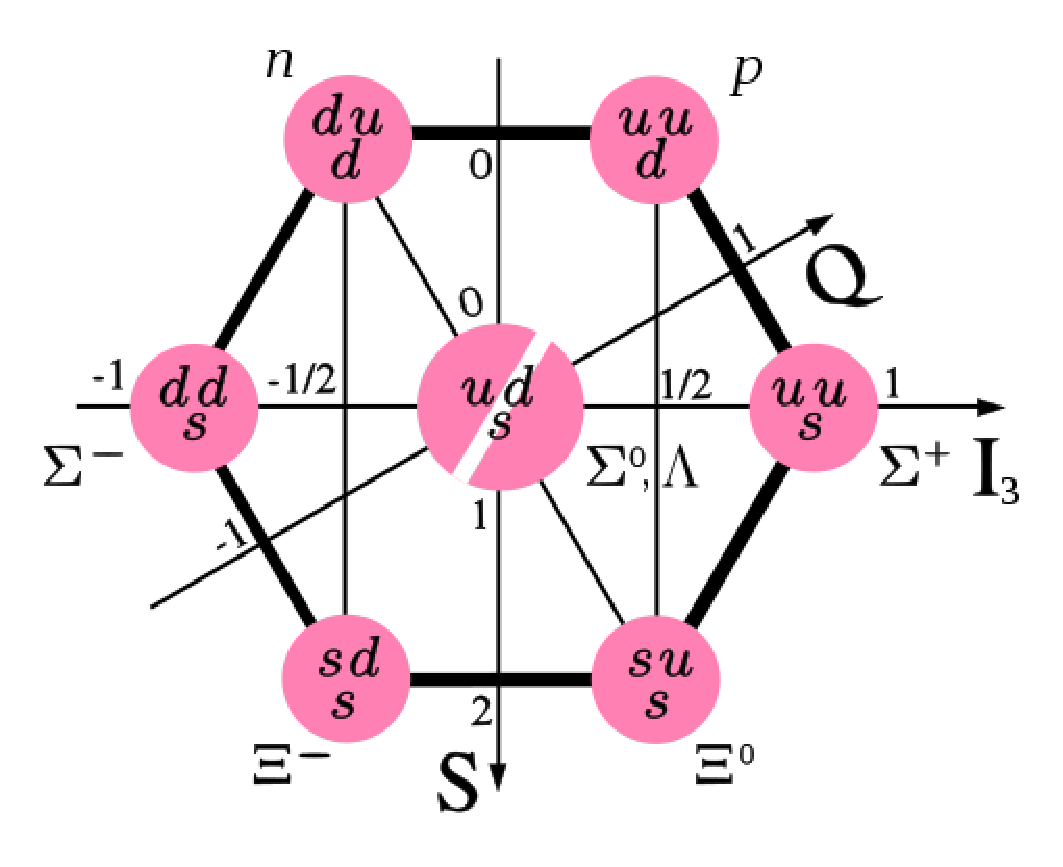
\includegraphics[scale=0.4]{pics/baryon_octet}
\end{center}
\caption{Barionski oktet.}
\label{fig:baryon_octet}
\end{figure}
Kod grupe \SU{2}, bilo spina, bilo izospina, definiciona reprezentacija
(izo)spina $\fhalf$ se obilato nalazi u prirodi. S druge strane,
u vrijeme nastanka "osmerostrukog puta," nije bila poznata nijedna
grupa čestica koja bi odgovarala definicionoj reprezentaciji grupe
\SU{3} --- tripletu. Da bi si pomogli u računima, Gell-Mann i
G. Zweig su postulirali tri hipotetske čestice koje je Gell-Mann nazvao
\emph{kvarkovi}, s današnjim imenima $u$ (\emph{up}, gornji), $d$
(\emph{down}, donji) i $s$ (\emph{strange}, strani, čudni) od kojih
je bilo moguće izgraditi sve druge tada poznate čestice. Na slici
\ref{fig:baryon_octet} je vidljiv i kvarkovski sastav čestica barionskog
okteta.
Originalno se mislilo da su kvarkovi samo pomagalo prilikom računa,
no s vremenom su i sami kvarkovi opaženi u eksperimentima, a kasnije
su otkrivena još i tri dodatna kvarka, $c$, $b$ i $t$. Ovi dodatni
kvarkovi u načelu omogućuju i daljnje proširenje simetrije
na \SU{4} itd., ali zbog velikih razlika u masama ovih dodatnih kvarkova
te su simetrije jako narušene i nisu od takve koristi kao
izospin i \SU{3}.
Svaki od šest vrsta kvarkova (poznatih i kao šest "okusa") 
dolazi u tri varijante (poznate kao tri "boje"), tako da kvarkova
zapravo ima 18. Od velike je važnosti simetrija koja međusobno
transformira tri bojna stanja kvarka i koja također ima grupno-teorijska
svojstva grupe \SU{3}. 
Treba dobro razlikovati simetriju \SU{3} okusa, koja je samo približna
simetrija prirode narušena različitim nabojima i masama kvarkova
i egzaktnu simetriju \SU{3} boje. Kad postoji opasnost zabune,
koriste se oznake $\SU{3}_{\mathrm{F}}$ i $\SU{3}_{\mathrm{C}}$.


\section{SU(3) tenzori}

Za grupu \SU{2} smo identificirali sve njene ireducibilne reprezentacije
razmatrajući isključivo same generatore grupe i njihove komutacijske relacije.
Slična procedura je u načelu moguća i za \SU{3}, ali mi ćemo se ovdje osloniti
na intuitivniji pristup koji se fokusira na same objekte na koje operatori
reprezentacije djeluju. Ti su objekti \SU{3} tenzori raznih rangova
(prisjetite se definicije \ref{def:tenzor} i diskusije iza primjera
\ref{pr:tenzorvodljivosti})
i ta metoda razmatranja reprezentacija se onda naziva "tenzorska."
Postupke i rezultate ćemo prikazati na razini recepta, bez detaljnog dokazivanja.


Pogledajmo prvo tenzorski pristup reprezentacijama grupe \SU{2}.
Sve ireducibilne reprezentacije te grupe mogu se dobiti
višestrukim direktnim množenjem fundamentalne dvodimenzionalne reprezentacije
(dubleta) sa samom sobom\footnote{Podsjećamo da se u žargonu izraz
    "reprezentacija" koristi i za skup operatora homomorfan grupi i za vektorski prostor
    na kojem ti operatori djeluju. U ovom odjeljku ćemo obično
misliti na ovo drugo.}. (Fizikalno govoreći, kombinirajući dovoljan broj
sustava spina $1/2$ možemo dobiti sustav bilo kojeg spina.). Npr. ukoliko
fundamentalni dublet označimo kao
$\psi^a$, $a=1,2$, gdje je 
\begin{displaymath}
 \psi^1 \equiv \ket{\fhalf,\fhalf} \;, \quad \psi^2
\equiv \ket{\fhalf, -\fhalf} \;,
\end{displaymath}
onda direktan produkt tog dubleta sa samim sobom daje četiri stanja:
\begin{displaymath}
 \psi^{11}\equiv \psi^1 \otimes \psi^1 \;, \quad \psi^{12} \;, \quad \psi^{21} \;
 \quad \text{i} \quad \psi^{22} \;.
\end{displaymath}
No znamo da su ireducibilne reprezentacije od \SU{2} zapravo 
\emph{antisimetrični} singlet
\begin{displaymath}
   \psi^{12} - \psi^{21}
\end{displaymath}
i \emph{simetrični} triplet
\begin{displaymath}
 \psi^{11},  \psi^{12} + \psi^{21}, \psi^{22} \;.
\end{displaymath}
Ova potreba da se ireducibilne reprezentacije formiraju 
simetrizacijom i antisimetrizacijom je djelomično rasvijetljena
u odjeljku \ref{sect:sfericniVSkartezijevi} gdje je pokazano 
kako se simetrične i antisimetrične komponente 
tenzora ne miješaju pri transformacijama.
Na isti način, direktnim množenjem i (anti)simetriziranjem
fundamentalnih trodimenzionalnih reprezentacija grupe \SU{3} moguće
je konstruirati sve njene ireducibilne reprezentacije. Kao prvo, potrebno je uočiti da
\SU{3} ima \emph{dvije} neekvivalentne trodimenzionalne reprezentacije,
čiji operatori su povezani kompleksnom konjugacijom: $U(g)$ i
$U(g)^*$. (Za \SU{2} grupu su odgovarajuće dvodimenzionalne reprezentacije ekvivalentne
pa je dovoljno raditi samo s jednim fundamentalnim dubletom, vidi
zadatak \thechapter.\ref{zad:su2dublet}.)
Da bismo razlikovali te dvije reprezentacije, odgovarajuće vektore
ćemo označavati s gornjim ili donjim indeksom:
\begin{align}
 3&: \qquad  \psi^a \to \psi^{'a} = \tensor{U}{^a_b} \, \psi^{b} \;, \\
 3^*&: \qquad  \psi_a \to \psi^{'}_a = \tensor{U}{^*_a^b} \, \psi_{b} \;.
\label{eq:su3fundamental}
\end{align}
Reprezentaciju 3 obično zovemo \emph{triplet}, a
reprezentaciju $3^*$ \emph{antitriplet}.
Direktnim množenjem ovih dviju  reprezentacija dobivamo 
tenzore višeg ranga, $\psi^{ab\cdots}_{r\cdots}$, koji
se transformiraju kao:
\begin{equation}
  \psi^{ab\cdots}_{r\cdots} \to 
 \tensor{U}{^{a}_{a'}} \tensor{U}{^{b}_{b'}} \cdots \tensor{U}{^*_r^{r'}} \cdots
  \psi^{a'b'\cdots}_{r'\cdots} \;.
\label{eq:mntensor}
\end{equation}

Promotrimo sada direktni produkt 3 i $3^*$ reprezentacija tj.
tenzor $\psi^a \psi_b \equiv \psi^{a}_{b}$.
Kao prvo, trag tog tenzora $\psi^a \psi_a$ je invarijantan na \SU{3}
transformacije
\begin{equation}
 \psi^a \psi_a \to \tensor{U}{^{a}_{b}}\tensor{U}{^*_a^c} \psi^b \psi_c
= \tensor{(U^\dagger U)}{^c_b} \psi^b \psi_c
= \tensor{\delta}{^c_b} \psi^b \psi_c = \psi^b \psi_b \,,
\end{equation}
(koristili smo $\tensor{U}{^*_a^c}=\tensor{U}{^\dagger^c_a}$) 
što znači da je taj trag  tenzor ranga 0.
To nam sugerira da tenzor $\psi^a \psi_b$ rastavimo 
 dio s tragom nula i sam trag
\begin{equation}
\psi^a \psi_b = \left(\psi^a \psi_b - \frac{1}{3}
\tensor{\delta}{^a_b}\psi^c \psi_c \right) +
\frac{1}{3} \tensor{\delta}{^a_b} \psi^c \psi_c  \;.
\label{eq:rastav3c3tensor}
\end{equation}
Daljnje rastavljanje prvog člana odvajanjem simetričnog i antisimetričnog
dijela tenzora nije moguće jer gornji i donji indeks
nisu ekvivalentni. Kako smo ustanovili da je trag ranga 0,
dakle singlet, imamo konačno:
\begin{equation}
  3 \otimes 3^* = 8 \oplus 1 \;.
\label{eq:rastav3c3}
\end{equation}

To da je trag invarijantan je očito i iz toga što nema
"slobodnog" indeksa na koji bi djelovao operator transformacije
$\tensor{U}{^{a}_{b}}$. Postoje međutim i važni tenzori
viših rangova koji su također invarijantni.
Prvi je Kroneckerov simbol $\tensor{\delta}{^a_b}$ koji je \SU{3} 
tenzor ranga 2 (usporedi u (\ref{eq:rastav3c3tensor})) koji je invarijantan jer
\begin{equation*}
\tensor{\delta}{^a_b} \to  \tensor{U}{^a_c}
\tensor{U}{^*_b^d} \tensor{\delta}{^c_d} = 
\tensor{U}{^a_c} \tensor{U}{^*_b^c} = \tensor{\delta}{^a_b} \;.
\end{equation*}
Na sličan način se je moguće uvjeriti da su Levi-Civita
tenzori $\epsilon^{abc}$  i $\epsilon_{abc}$ 
također invarijantni.
Na primjer, 
\begin{equation}
    \epsilon^{abc} \to     
     \tensor{U}{^a_d}
     \tensor{U}{^b_e}
     \tensor{U}{^c_f}\epsilon^{def} 
     = \det U \epsilon^{abc} = \epsilon^{abc} \,,
\end{equation}
gdje smo upotrijebili svojstvo iz zadatka \ref{zad:levicivita}.
Značaj Levi-Civita tenzora je da se pomoću
njih mogu ``spuštati i dizati indeksi'' drugih tenzora.
Npr. promotrimo antisimetričnu komponentu tenzora $\psi^{ab}$,
koju dobijemo kao $\tensor{\psi}{^{[ab]}} \equiv (\psi^{ab}-\psi^{ba})/2$.
Ona očito ima samo tri nezavisna elementa (slično kao
antisimetrična $3\times 3$ matrica). Kontrakcijom s 
Levi-Civita tenzorom možemo tu činjenicu učiniti eksplicitnom
i pokazati da je $\tensor{\psi}{^{[ab]}}$ ekvivalentan
antitripletu $\psi_a$:
\begin{equation}
  \psi_a = \epsilon_{abc} \tensor{\psi}{^{bc}}
\label{eq:spustanjeindeksa}
\end{equation}
Usput, Levi-Civita tenzor invarijantan na 
djelovanje \SU{2} grupe ima samo
dva indeksa $\epsilon_{ij}$, pa podižući i spuštajući
indekse ne mijenja rang tenzora, te se i tako vidi
da su u \SU{2} dublet $\psi^{i}$ i antidublet
$\psi_{i} = \epsilon_{ij}\psi^{j}$ ekvivalentni i da
u \SU{2} općenito ne moramo razlikovati položaje indeksa.

\begin{primjer}[$3\otimes 3$]
Kako triplet i antitriplet nisu ekvivalentni, $3\otimes 3
\neq 3\otimes 3^*$. Kako su u
$3\otimes 3 = \psi^a \psi^b$ oba indeksa istog tipa,
možemo razdvojiti simetrični i antisimetrični dio ovog
tenzora koji su svaki za sebe ireducibilni,
\begin{align}
\psi^a \psi^b &= \fhalf (\psi^a\psi^b + \psi^b \psi^a)
               + \fhalf (\psi^a\psi^b - \psi^b \psi^a) \\
              &\equiv \psi^{(ab)} + \psi^{[ab]}
\end{align}
Prvi, potpuno simetrični član, ima šest nezavisnih komponenata
(broj nezavisnih elemenata simetrične 3$\times$3 matrice) i
predstavlja sekstuplet (6) reprezentaciju, dok smo gore
vidjeli da je $\psi^{[ab]}$ ekvivalentan antitripletu
$\psi_c$. 

Podsjetimo se da smo u odjeljku \ref{sect:tenzorskioperatori},
simetrične 6-dim operatore dodatno reducirali na jednodimenzionalni
trag i 5-dim simetrični dio s tragom nula.  Ovdje to ne možemo učiniti
jer na raspolaganju imamo samo 
$\tensor{\delta}{^a_b}$ i $\tensor{\delta}{_a^b}$ kao \SU{3} invarijante, 
ali ne i $\delta^{ab}$! (U odjeljku \ref{sect:tenzorskioperatori}
to nije bio problem jer u
\SU{2} ne moramo paziti na razliku između gornjih i donjih indeksa.)
Stoga je sekstuplet $\psi^{(ab)}$ ireducibilan.

Dakle, konačni rezultat je
\begin{equation}
 3 \otimes 3 = 6 \oplus 3^*
\label{eq:33eq63}
\end{equation}
\end{primjer}

\begin{primjer}[$3\otimes 3\otimes 3$]
Koristimo prvo rezultat iz zadnjeg primjera:
\begin{equation}
3\otimes 3\otimes 3 = 3 \otimes (6 \oplus 3^*)
= (3 \otimes 6) \oplus (3 \otimes 3^*) \;.
\end{equation}
Drugi član već znamo iz (\ref{eq:rastav3c3}), a prvi je
direktan umnožak seksteta $\psi^{(ab)}$ i tripleta $\psi^{c}$.
Iz tog umnoška možemo izdvojiti potpuno simetričnu komponentu:
\begin{equation}
\psi^{(ab)}\psi^{c} = \psi^{(abc)} + \text{ostatak} \;. 
\label{eq:6x3}
\end{equation}
Tenzor $\psi^{(abc)}$ je totalno simetrični
tenzor ranga 3. Broj njegovih nezavisnih komponenata može
se odrediti i izravnim brojanjem. Prvo, postoji
samo jedna nezavisna komponenta sa sva tri različita
indeksa, npr. $\psi^{123}$, i sve ostale su joj jednake:
$\psi^{123} = \psi^{213} = \psi^{312} = \ldots$. Nezavisnih komponenata
s dva ista indeksa i trećim različitim ima šest, npr.
$\psi^{112}, \psi^{113}, \psi^{221}, \psi^{223},
\psi^{331}$ i $\psi^{332}$. Imamo još i tri nezavisne
komponente sa sva tri indeksa ista (na "hiperdijagonali"
tenzora), $\psi^{111}$, $\psi^{222}$ i $\psi^{333}$, što sve skupa
čini ukupno 10 nezavisnih komponenata. Dakle, $\psi^{(abc)}$ je
dekuplet (10). Preostali dio u rastavu $3 \otimes 6$ ima
dimenziju $3\times6-10=8$ i odgovara oktetu (8). (Tu
zadnju ekvivalenciju nije lako pokazati ovom tenzorskom
metodom. Pokazat ćemo to u zadatku \thechapter.\ref{zad:3x3x3} 
metodom iz sljedećeg odjeljka.)
Dakle, konačni rezultat je
\begin{equation}
 3 \otimes 3 \otimes 3 = 10 \oplus 8 \oplus 8 \oplus 1
\label{eq:3x3x3}
\end{equation}
Ovaj primjer je od velikog fizikalnog značaja jer odgovara
mogućim kombinacijama triju lakih kvarkova koji čine
fundamentalni \SU{3} triplet
\begin{equation}
 \psi^{1}=u\;, \quad \psi^{2}=d \;, \quad \psi^{3} = s \;,
\end{equation}
Jedan od okteta, prikazan na slici \ref{fig:baryon_octet}, sadrži 
proton i neutron.
\end{primjer}

Tenzorske metode analize \SU{3} ireducibilnih reprezentacija, prikazane
u ovom odjeljku, su pogodne jer istovremeno pokazuju strukturu samih
\SU{3} objekata što je često od interesa u primjenama, gdje ti objekti
odgovaraju kvantnomehaničkim stanjima. Međutim, kako
dimenzije reprezentacija rastu, i s njima broj indeksa tenzora,
metoda postaje komplicirana. Jednostavnija za primjenu i općenitija
je metoda Youngovih dijagrama, koju predstavljamo u 
sljedećem odjeljku. Klasične reference za napredniji studij ovih
tenzorskih metoda i njihovih primjena na fiziku čestica
su \cite{Coleman:1985} i \cite{Georgi:1999}.


\section{SU(N) tenzori i Youngovi dijagrami}

Youngov dijagram je dijagram poput ovog
$$
\ydiagram{5,5,3,1}
$$
gdje je važno svojstvo konveksnosti prema dolje desno tj. da
je lijeva strana poravnata i da se broj polja u retcima
\emph{ne smanjuje} kako idemo odozgo prema dolje.
Dakle, sljedeći dijagrami \emph{nisu} ispravni Youngovi dijagrami.
$$
\ydiagram{2+1,3,3} \qquad  \qquad  \ydiagram{3,4,1}
$$
Youngov dijagram s $k$ polja je ekvivalentan \SU{N} tenzoru s
$k$ indeksa kojem su prvo indeksi koji odgovaraju pojedinim
retcima dijagrama simetrizirani, a zatim indeksi koji odgovaraju
pojedinim stupcima antisimetrizirani.
\begin{equation}
\ytableaushort{abc, de} \qquad \Longleftrightarrow \qquad
\psi^{[ad][be]c} \;.
\label{eq:tbltensor}
\end{equation}
Uočite da antisimetrizacija po stupcima pokvari simetriju po retcima.
Ukoliko je u ovom primjeru riječ o \SU{3} tenzoru, znamo da je par
antisimetriziranih gornjih indeksa ekvivalentan jednom donjem indeksu
nakon spuštanja pomoću Levi-Civita tenzora:
\begin{equation}
\SU{3}:\quad 
\ytableaushort{abc, de} \qquad \Longleftrightarrow \qquad
\psi^{[ad][be]c} \qquad \Longleftrightarrow \qquad
\psi^{c}_{fg} \;.
\label{eq:tbltensorsu3}
\end{equation}
Na sličan način možemo svaki tenzor (dakle svaku ireducibilnu reprezentaciju) prikazati
posebnim Youngovim dijagramom. Npr. u \SU{3}:
\begin{align}
\ydiagram{1} \qquad\qquad \psi^a \qquad\qquad 3  \\[2ex]
\ydiagram{1,1} \qquad\qquad \psi^{[ab]} \Leftrightarrow \psi_c  \qquad\qquad 3^*  \\[2ex]
\ydiagram{2} \qquad\qquad \psi^{(ab)}  \qquad\qquad 6  \\[2ex]
\ydiagram{1,1,1} \qquad\qquad \psi^{[abc]} \propto \epsilon^{abc} \qquad\qquad 1
\end{align}
U zadnjem redu smo iskoristili činjenicu da je potpuno antisimetrični tenzor s tri
indeksa nužno proporcionalan Levi-Civiti, što znači da je invarijantan i
da ga trebamo tretirati kao singlet tj. jedinični element u algebri
reprezentacija. Ekvivalentno, stupac s N polja
Youngovog dijagrama \SU{N} grupe možemo brisati. Dijagram s više od N polja
je naprosto nula jer npr. nije moguće napraviti potpuno antisimetrični tenzor
s četiri indeksa u \SU{3} gdje indeksi poprimaju
samo vrijednosti $1$, $2$ i $3$ pa dva od ta četiri indeksa nužno moraju
biti jednaka.

Pokažimo sada kako se
određuje dimenzija SU(N) reprezentacije reprezentirane 
nekim Youngovim dijagramom.
Youngov dijagram obrojčimo na dva sljedeća načina:

Prvi način: U lijevi gornji kut upišemo $N$ (za \SU{N}), i ostatak
reda obrojčimo s sukcesivno rastučim brojevima. Slijedeći red isto,
ali počnemo s $N-1$. I tako dalje.
\begin{displaymath}
\ytableausetup{boxsize=2.5em}
\begin{ytableau} 
\scriptstyle N &\scriptstyle N+1 &\scriptstyle N+2 \\
\scriptstyle N-1 &\scriptstyle N \\
\scriptstyle N-2 \\
\scriptstyle N-3
\end{ytableau}
\end{displaymath}

Drugi način: svako polje dijagrama dobije broj određen ``pravilom kuke''.
Kuka je linija koja od tog polja ide desno u beskonačnost i od tog
istog polja dolje u beskonačnost. Broj polja preko kojih
kuka prolazi upišemo u dato polje. Postupak ponavljamo za sva polja.

\begin{center}
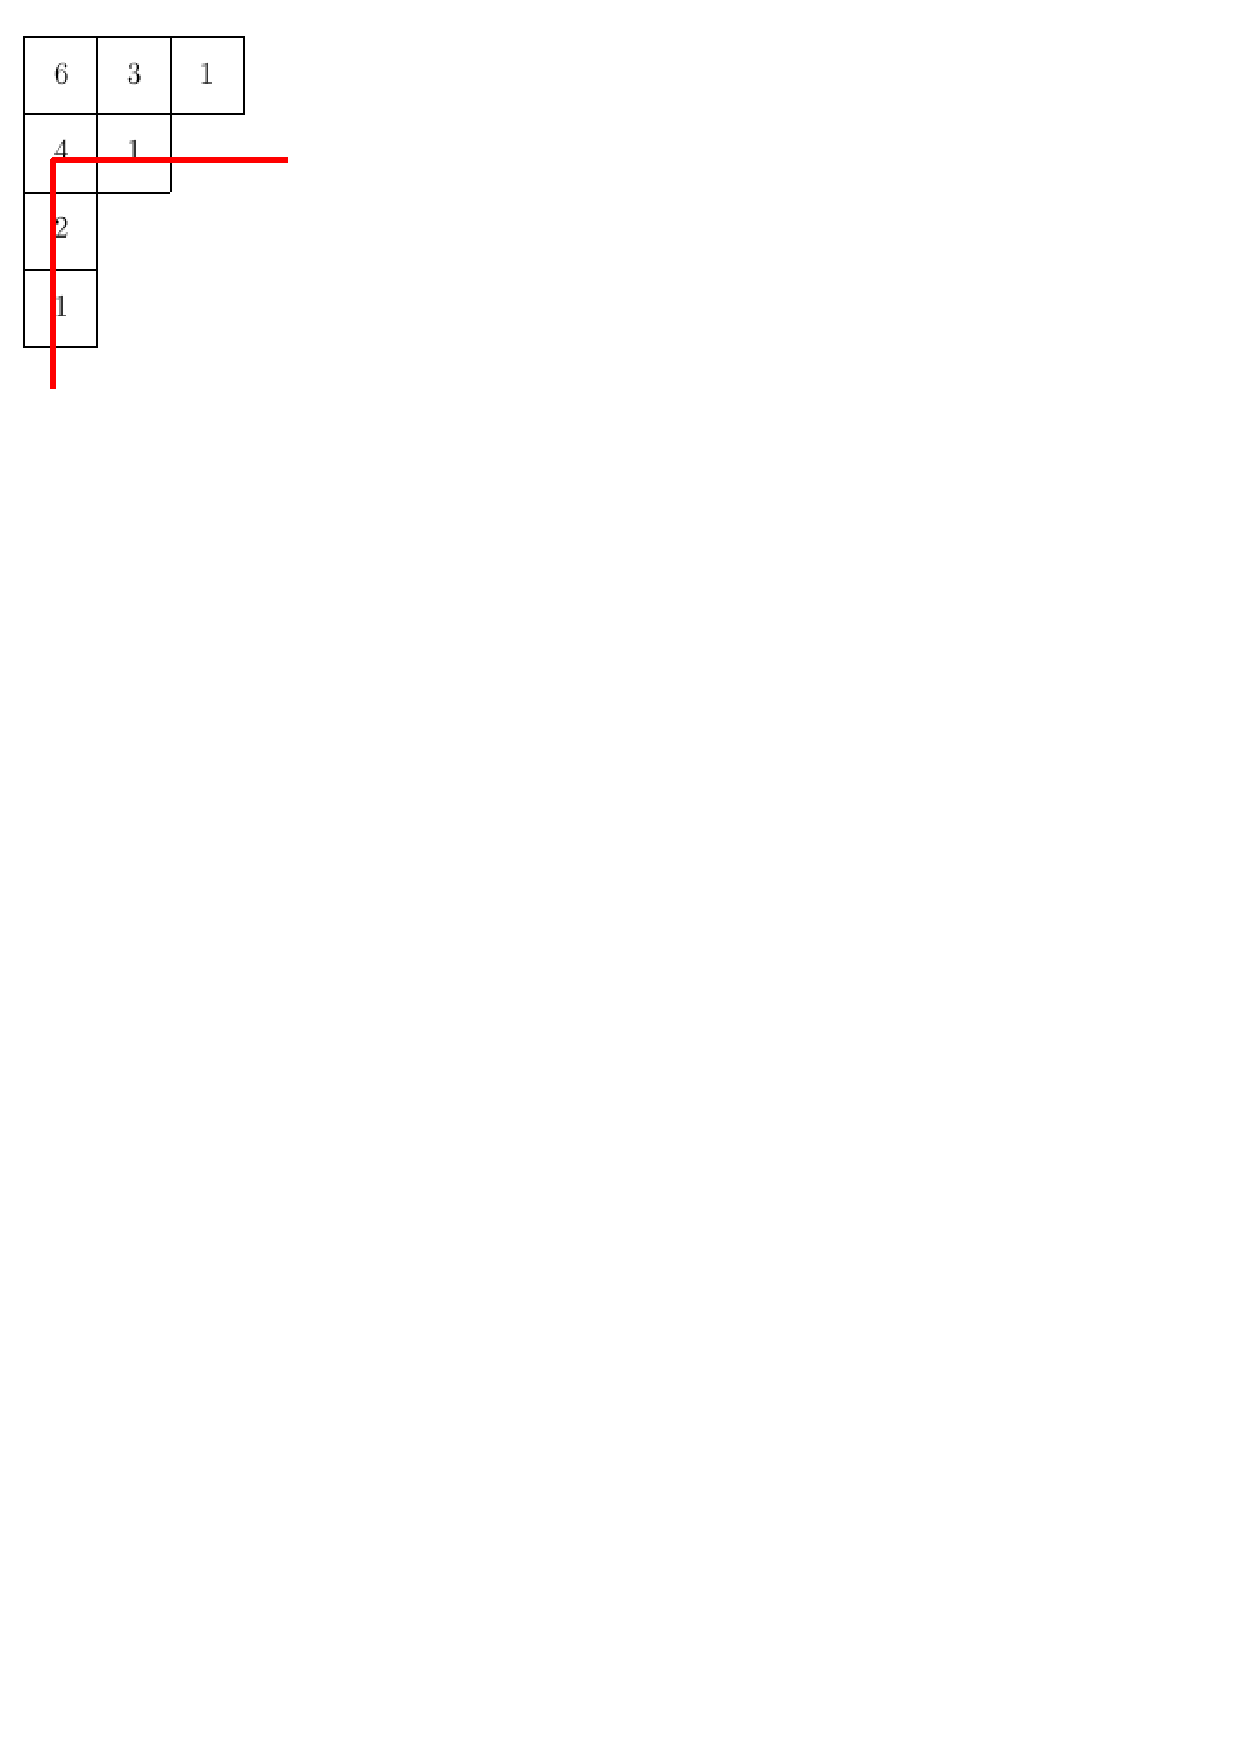
\includegraphics[scale=0.8]{pics/kukat}
\end{center}

Sada pomnožimo posebno sve brojeve u dijagramu obrojčenom na prvi način i
posebno sve brojeve u dijagramu obrojčenom na drugi način. Dimenzija
ireducibilne reprezentacije je omjer ta dva broja.
Evo tri primjera iz \SU{3}:
\begin{displaymath}
\ytableausetup{boxsize=normal}
\SU{3}: \qquad \frac{\ytableaushort{34,2}}{\ytableaushort{31,1}} = \frac{24}{3}= 8
\qquad
\frac{\ytableaushort{3}}{\ytableaushort{1}} = \frac{3}{1}= 3
\qquad
\frac{\ytableaushort{3,2}}{\ytableaushort{2,1}} = \frac{6}{2}= 3^*
\end{displaymath}
U zadnjem od gornja tri primjera smo se oslonili na informacije ranije dobivene
tenzorskim metodama da bi odredili da je zadnja reprezentacija zapravo
antitriplet, a ne triplet. Navedimo još neke primjere:
\begin{displaymath}
\SU{3}: \qquad \frac{\ytableaushort{34}}{\ytableaushort{21}} = \frac{12}{2}= 6
\qquad
\frac{\ytableaushort{345}}{\ytableaushort{321}} = \frac{60}{6}= 10
\end{displaymath}

\begin{displaymath}
\SU{3}: \qquad \frac{\ytableaushort{345,234}}{\ytableaushort{432,321}} = 10
 \qquad 
\frac{\ytableaushort{3456,23}}{\ytableaushort{5421,21}} = 27
\end{displaymath}

\begin{displaymath}
\SU{5}: \qquad \frac{\ytableaushort{56,4}}{\ytableaushort{31,1}} = 40
\end{displaymath}


Rastav direktnog produkta dvije \SU{N} ireducibilne reprezentacije na direktan zbroj
(Clebsch-Gordanov razvoj) izvodi se množenjem odgovarajućih
Youngovih dijagrama, $T_1$ i $T_2$, na sljedeći način. Polja u desnom
dijagramu ozačimo slovima: polja prvog retka
s $a$, polja drugog retka s $b$ i tako dalje:

\begin{displaymath}
\renewcommand{\arraystretch}{2}
\begin{array}{c}
\ydiagram{2,1,1} \\ T_1
\end{array}
 \qquad \otimes \qquad 
\begin{array}{c}
\ytableaushort{aaa,bb,c} \\ T_2
\end{array}
\end{displaymath}

Sada prebacujemo polja s $T_2$ na $T_1$, jedno po jedno, redak
po redak, odozgo prema dolje, na sve moguće načine, tako da
budu zadovoljena sljedeća pravila.
\begin{enumerate}
\item $T_1$ je u svakom trenutku ispravni Youngov dijagram.
\item Polja s istim slovom ne smiju biti u istom stupcu.
 (Posljedica činjenice da su stupci antisimetrizirani.)
\item Za svako polje nastajućeg tenzora je definiran $n_a$
kao broj polja s indeksom $a$ iznad i desno od njega.
Isto tako $n_b$ itd. Mora biti: $n_a \ge n_b \ge n_c$.
\end{enumerate}
Na kraju 
\begin{itemize}
\item Maknemo stupce s $N$ polja. (Jer je totalno
antisimetrični tenzor s $N$ indeksa proporcionalan
s $\epsilon^{a_1 a_2 \cdots a_N}$ i time \SU{N}
invarijanta.)
\item Dva dijagrama istog oblika  odgovaraju
posebnim ireducibilnim reprezentacijama samo ako se razlikuju po razmještaju
slova $a,b,\dots$. U suprotnom jednog maknemo.
\end{itemize}

\begin{primjer}[$8 \otimes 8$ u \SU{3}]
\begin{displaymath}
\ydiagram{2,1} \quad\otimes\quad \ytableaushort{aa,b} \quad = 
\end{displaymath}
Jedno {\ytableausetup{smalltableaux}$\ytableaushort{a}$
\ytableausetup{nosmalltableaux}} se može premjestiti na
$T_1$ na tri različita načina
\begin{displaymath}
\left( 
\ytableaushort{\none \none a,\none} * {3, 1}
\quad \oplus \quad
\ytableaushort{\none \none, \none a} * {2, 2}
\quad \oplus \quad
\ytableaushort{\none \none, \none, a} * {2, 1, 1}
\right) 
\quad\otimes\quad \ytableaushort{a,b} \quad = 
\end{displaymath}
Sad premještamo drugo {\ytableausetup{smalltableaux}$\ytableaushort{a}$
\ytableausetup{nosmalltableaux}}:
\begin{align*}
\left( 
\ytableaushort{\none \none a a,\none} * {4, 1}
\quad\oplus\quad 
\ytableaushort{\none \none a, \none a} * {3, 2}
\quad\oplus\quad 
\ytableaushort{\none \none a, \none, a} * {3, 1, 1}
\right)& 
\quad\otimes\quad \ytableaushort{b}  \\
\quad\oplus\quad\left( 
\ytableaushort{\none \none a,\none a} * {3, 2}
\quad\oplus\quad 
\ytableaushort{\none \none, \none a, a} * {2, 2, 1}
\right)& 
\quad\otimes\quad \ytableaushort{b}  \\
\quad\oplus\quad\left( 
\ytableaushort{\none \none a,\none, a} * {3, 1, 1}
\quad\oplus\quad 
\ytableaushort{\none \none, \none a, a} * {2, 2, 1}
\right)& 
\quad\otimes\quad \ytableaushort{b} \quad=
\end{align*}
Tu iznad imamo tri dijagrama u duplikatu pa po jedan maknemo:
\begin{displaymath}
\left( 
\ytableaushort{\none \none a a,\none} * {4, 1}
\quad\oplus\quad 
\ytableaushort{\none \none a, \none a} * {3, 2}
\quad\oplus\quad 
\ytableaushort{\none \none a, \none, a} * {3, 1, 1}
\quad\oplus\quad 
\ytableaushort{\none \none, \none a, a} * {2, 2, 1}
\right) 
\quad\otimes\quad \ytableaushort{b} \quad=
\end{displaymath}
\begin{multline*}
\ytableaushort{\none \none a a,\none b} * {4, 2}
\quad\oplus\quad 
\ytableaushort{\none \none a a,\none, b} * {4, 1, 1}
\quad\oplus\quad 
\ytableaushort{\none \none a, \none a b} * {3, 3} \\
\quad\oplus\quad 
\ytableaushort{\none \none a, \none a, b} * {3, 2, 1}
\quad\oplus\quad 
\ytableaushort{\none \none a, \none b, a} * {3, 2, 1}
\quad\oplus\quad 
\ytableaushort{\none \none , \none a, a b} * {2, 2, 2}
\end{multline*}
Primijetite da ovdje nismo kreirali sljedeće dijagrame koji
bi narušavali gornja pravila:
\begin{displaymath}
\ytableaushort{\none \none a a b, \none} * {5, 1}
\qquad \text{i} \qquad
\ytableaushort{\none \none a, \none, a, b} * {3, 1,1, 1}
\end{displaymath}
Sada maknemo sve stupce s tri polja (\SU{3} invarijante)
i dobijemo konačno:
\begin{equation*}
\ytableaushort{\none \none a a,\none b} * {4, 2}
\quad\oplus\quad 
\ytableaushort{\none a a} * {3}
\quad\oplus\quad 
\ytableaushort{\none \none a, \none a b} * {3, 3}
\quad\oplus\quad 
\ytableaushort{\none a, a} * {2, 1}
\quad\oplus\quad 
\ytableaushort{\none a,  b} * {2, 1}
\quad\oplus\quad 
1
\end{equation*}
Dimenzije ireducibilnih reprezentacija za sve ove dijagrame smo već odredili pa
očitavamo konačni rezultat
\begin{equation}
8 \otimes 8 = 27 \oplus 10 \oplus 10 \oplus 8 \oplus 8 \oplus 1
\label{eq:8x8}
\end{equation}
(Zgodno je uočiti da je postupak jednostavniji ako pri množenju
kao desni uzmemo Youngov dijagram s manje polja.)

\end{primjer}

\subsection*{Zadaci}

\begin{enumerate}[label=\arabic{chapter}.\arabic*.]

\item Ako pretpostavimo očuvanje izospina, koja su moguća izospinska
stanja (ukupni izospin i treća komponenta ukupnog izospina) pri
raspršenju protona na

 \begin{description} \item[a)] $\pi^+$
                     \item[b)] $\pi^0$
                     \item[c)] $\pi^-$. \end{description}


\item \label{zad:fabc}
Pokažite da su, zahvaljujući komutacijskim relacijama i relaciji (\ref{eq:SU3norm}),
strukturne konstante $f_{ABC}$, grupe SO(3) potpuno antisimetrične u
svim indeksima.

\item \label{zad:su2dublet}
Pokažite da je za \SU{2}  $2^* = 2$ tj. da su fundamentalni dublet i
antidublet ekvivalentni, tako da pokažete da je operator $C$
\begin{displaymath}
  C = U(R(\hat{y},\theta=\pi)) = \exp\left(-\frac{i}{\hbar} J_2 \pi\right) \;
\end{displaymath}
operator koji povezuje 2 i $2^*$:
\begin{align*}
C \sigma_i C^{-1}& = - \sigma_{i}^* \\
C U(g) C^{-1}& = U(g)^*
\end{align*}


\item \label{zad:3x3x3}
Izračunajte Clebsch-Gordanov razvoj u \SU{3} grupi za
\begin{itemize}
\item $3^* \otimes 3$
\item $3 \otimes 3$
\item $3 \otimes 3 \otimes 3$
\end{itemize}

\item Izračunajte Clebsch-Gordanov razvoj u \SU{6} grupi za
\begin{itemize}
\item $6 \otimes 6^*$
\item $6 \otimes 6 \otimes 6$
\end{itemize}

\end{enumerate}
